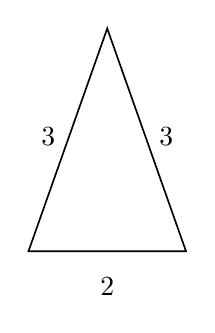
\begin{tikzpicture}[x=1cm,y=1cm,font=\normalsize,
 geometry edge/.style={solid,line width=.6pt},
 geometry mark/.style={solid,line width=.6pt},
 geometry label/.style={font=\normalsize,inner sep=2pt}]
\coordinate (T1) at (0,2.8284);
\coordinate (T2) at (-1,0);
\coordinate (T3) at (1,0);
\draw[geometry edge] (T1)--(T2)--(T3)--cycle;
\node[font=\normalsize] at (-0.75,1.45) {$3$};
\node[font=\normalsize] at (0.75,1.45) {$3$};
\node[font=\normalsize] at (0,-0.45) {$2$};
\end{tikzpicture}
